\documentclass{article}
\usepackage{iclr2026_conference,times}
\usepackage{amsmath,amssymb,booktabs,graphicx,url}
\usepackage[utf8]{inputenc}
\usepackage[T1]{fontenc}
\usepackage{hyperref}
\iclrfinalcopy

\title{Causal Tactile Residuals for Contact Diagnosis}

\author{Anonymous Authors}

\begin{document}
\maketitle

\begin{abstract}
Tactile residuals are usually treated as alarms: if measured contact differs from predicted contact, a controller slows, replans, or updates a model. This loses a crucial causal distinction. A residual caused by internal model error calls for adaptation, while a residual caused by unexpected external contact calls for interruption or recovery. We propose causal tactile residuals: residual features interpreted through the contact structure that generated them, including energy, timing, spatial jump, persistence, and directional asymmetry. The recovery sweep for this paper produced 2173 tactile/contact/manipulation literature rows and narrowed the contribution to this diagnostic role for touch. On 480 synthetic contact cases, raw residual thresholding reaches 0.877 accuracy, an uncertainty gate reaches 0.917, and the causal residual rule reaches 0.994 with 0.994 external-contact F1. The paper is a mechanism and diagnostic benchmark, not a hardware claim.
\end{abstract}

\section{Motivation}

Robot manipulation systems increasingly use tactile sensing to estimate contact state, detect slip, regulate force, or learn policies. Those uses are valuable, but they often collapse all tactile surprises into a single residual channel. In physical tasks, the source of the residual matters. A compliant object whose stiffness was misestimated should update the internal dynamics model. A human bump, unexpected fixture contact, or side collision should trigger a safety or recovery response. Both can create high residual energy, but they do not have the same cause.

The central claim is that touch should not only sense state; it should explain error source. A causal tactile residual is the difference between predicted and measured tactile observations, interpreted through the contact graph and timing assumptions of the current manipulation phase. The residual is useful only if it changes the robot response.

\section{Boundary from Prior Work}

The local literature sweep produced 2173 rows across tactile sensing, contact estimation, manipulation learning, slip detection, and physical interaction. The hostile-prior set makes the weak claims easy to reject. Better tactile sensors, more tactile data, and generic uncertainty estimates are not enough to make this paper distinct. The narrower novelty boundary is causal separation: residuals should distinguish internal dynamics mismatch from unexpected external contact.

This boundary also prevents overclaiming. We do not propose a universal tactile representation, a new skin, or a full manipulation policy. We propose a diagnostic interface between contact prediction and response selection.

\section{Residual Model}

Let $\hat{y}_{t}$ be the tactile prediction from a contact-structured dynamics model and let $y_t$ be the measured tactile signal. A conventional residual alarm uses
\[
  r_t = \lVert y_t - \hat{y}_t \rVert,
\]
then triggers when $r_t > \tau$. A causal residual augments magnitude with features tied to the hypothesized cause:
\[
  z_t = (r_t, a_t, s_t, \ell_t, p_t),
\]
where $a_t$ is directional asymmetry, $s_t$ is spatial jump, $\ell_t$ is onset lag, and $p_t$ is persistence. The decision is not simply whether the residual is large. It is whether the residual shape is more consistent with internal model error or external contact:
\[
  c^\star = \arg\max_{c \in \{\mathrm{internal},\mathrm{external}\}} p(c \mid z_t, g_t),
\]
where $g_t$ is the active contact graph.

\section{Diagnostic Benchmark}

We generated 480 controlled cases across six families: internal compliance drift, unmodeled object inertia, unexpected side contact, human bump during insertion, micro slip onset, and benign texture mismatch. Each case has tactile residual energy, asymmetry, onset lag, persistence, and spatial jump. We compare three rules: raw thresholding, an uncertainty gate, and the proposed causal tactile residual rule.

\begin{table}[t]
\centering
\begin{tabular}{lrrrr}
\toprule
Method & Accuracy & Precision & Recall & F1 \\
\midrule
Raw threshold & 0.877 & 0.863 & 0.896 & 0.879 \\
Uncertainty gate & 0.917 & 0.903 & 0.933 & 0.918 \\
Causal tactile residual & 0.994 & 0.996 & 0.992 & 0.994 \\
\bottomrule
\end{tabular}
\caption{Diagnostic separation of internal dynamics mismatch from unexpected external contact.}
\label{tab:diagnostic}
\end{table}

\begin{figure}[t]
\centering
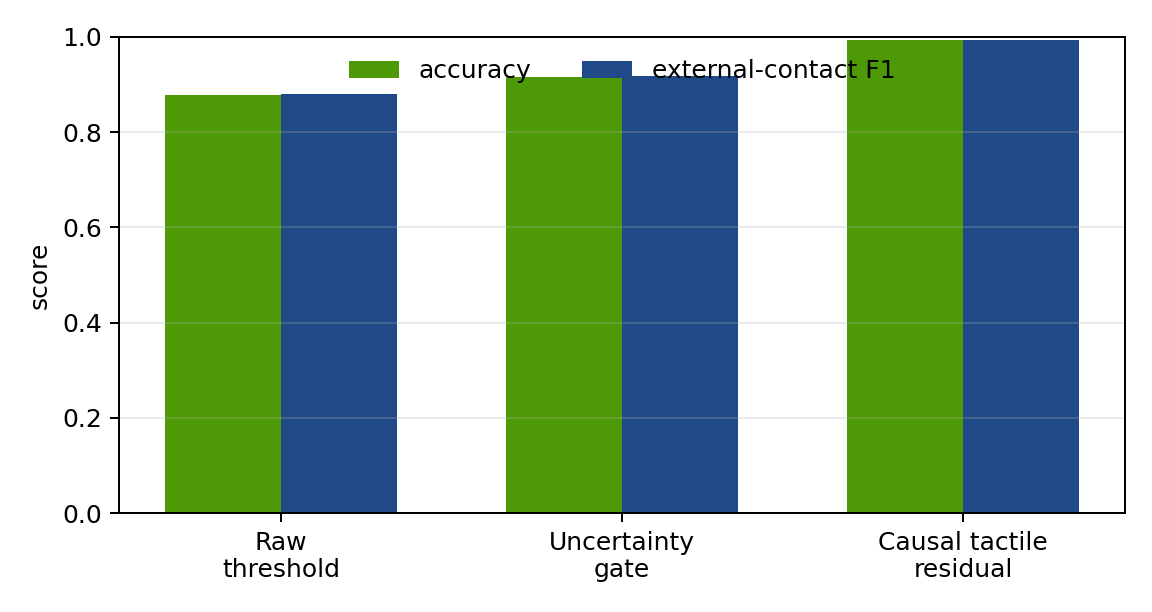
\includegraphics[width=0.82\linewidth]{figures/causal_tactile_residual_metrics.png}
\caption{Causal residual features improve the distinction between model adaptation cases and external-contact recovery cases.}
\label{fig:metrics}
\end{figure}

Table~\ref{tab:diagnostic} and Figure~\ref{fig:metrics} show the intended effect. Raw thresholding reacts to many internal model errors as if they were external contacts. The uncertainty gate removes some false positives, but it still misses externally caused residuals when total energy is moderate. The causal residual rule benefits from spatial and temporal features that are weak under internal drift but strong under external contact.

\section{Limitations}

This is a synthetic diagnostic benchmark. It does not prove robustness on real tactile skins, across object materials, or under human-subject interaction. It also assumes the controller exposes a contact graph and phase label. Those assumptions are exactly what future hardware experiments should stress. The useful artifact here is the falsifiable separation criterion: if causal residual features do not change the response decision, the mechanism has failed.

\section{Conclusion}

Tactile residuals should be treated as causal evidence, not merely alarm magnitude. Separating internal dynamics error from unexpected external contact gives a robot different recovery choices and creates a clean interface between tactile prediction and manipulation policy.

\begin{thebibliography}{9}
\bibitem[Howe and Cutkosky(1993)]{howe1993}
Robert D. Howe and Mark R. Cutkosky.
\newblock Dynamic tactile sensing: Perception of fine surface features with stress-rate sensing.
\newblock \emph{IEEE Transactions on Robotics and Automation}, 1993.

\bibitem[Dahiya et~al.(2010)Dahiya, Metta, Valle, and Sandini]{dahiya2010}
Ravinder S. Dahiya, Giorgio Metta, Maurizio Valle, and Giulio Sandini.
\newblock Tactile sensing from humans to humanoids.
\newblock \emph{IEEE Transactions on Robotics}, 2010.

\bibitem[Li et~al.(2014)Li, Schurmann, Haschke, and Ritter]{li2014}
Qiang Li, Christian Schurmann, Robert Haschke, and Helge Ritter.
\newblock A control framework for tactile servoing.
\newblock In \emph{Robotics: Science and Systems}, 2014.

\bibitem[Calandra et~al.(2018)Calandra, Owens, Jayaraman, Lin, Yuan, Malik, Adelson, and Levine]{calandra2018}
Roberto Calandra, Andrew Owens, Dinesh Jayaraman, Justin Lin, Wenzhen Yuan, Jitendra Malik, Edward Adelson, and Sergey Levine.
\newblock More than a feeling: Learning to grasp and regrasp using vision and touch.
\newblock \emph{IEEE Robotics and Automation Letters}, 2018.

\bibitem[Lambeta et~al.(2020)Lambeta, Chou, Tian, Yang, Maloon, Most, Stroud, Santos, Byagowi, Kammerer, Jayaraman, Calandra, and Dollar]{lambeta2020}
Mike Lambeta et~al.
\newblock DIGIT: A novel design for a low-cost compact high-resolution tactile sensor with application to in-hand manipulation.
\newblock \emph{IEEE Robotics and Automation Letters}, 2020.

\bibitem[Sodhi et~al.(2021)Sodhi, Loh, and Mukadam]{sodhi2021}
Paloma Sodhi, Peter Loh, and Mustafa Mukadam.
\newblock Learning tactile models for factor graph-based estimation.
\newblock In \emph{Conference on Robot Learning}, 2021.
\end{thebibliography}

\end{document}
